\documentclass{article}
\usepackage[legalpaper, margin=1in]{geometry}
\usepackage[utf8]{inputenc}
\usepackage{hyperref}
\usepackage{graphicx}
\usepackage{float}
\usepackage{listings}
\usepackage{minted}
\usepackage{xcolor}
\usepackage{caption}
\definecolor{LightGray}{gray}{0.9}
\setminted{
	linenos=true,
	autogobble,
}
% Create a new environment for breaking code listings across pages.
\newenvironment{longlisting}{\captionsetup{type=listing}}{}

\title{MoTiVML Guideline Document}
\author{}
\date{}

\begin{document}

\maketitle
This is a guideline document for the MoTiVML language for modelling variability in robotic systems. This guideline document serves as a supporting artifact to the language as well as a form of verification for the language and its capabilities.

\noindent\rule{17cm}{0.4pt}

\label{guide:docs}
\section{Prerequisites}
    \begin{itemize}
        \item Ubuntu 20.04.3 LTS and above
        \item ROS installation. This application was developed and tested with ROS Neotic 1.15.9.
        \item Python3 installation
        \item C++ 11 or higher
    \end{itemize}

\section{Setup and Installation of MoTiVML}
\begin{itemize}
    \item Clone MoTiVML from \href{https://github.com/SergioGarG/sera-extension}{here} into catkin workspace.
    \item Go the MoTiVML workspace project directory and build the cloned project by typing catkin\_make and press enter on your keyboard.
\end{itemize}

\section{How To}
This section gives a step-by-step walkthrough of how MoTiVML can be used to instantiate a model/configuration, validate a model and can be linked with source code implementations. We also give a brief walkthrough of the MoTiVML console interface. Throughout our demonstrations in this guideline document, we will use a sample model of a robot that is shown in figure \ref{simplebot}. This graphical representation of a simple robot model will serve as our running example throughout this guideline document.

\begin{figure}[H]
	\caption{Graphical Model of a Simple Robot}
	\centering
	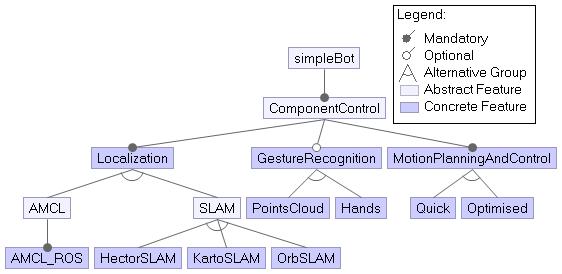
\includegraphics[width=\columnwidth]{images/simpleBot.png}
	\label{simplebot}
\end{figure}

\subsection{Instantiate a MoTiVML Model}
\begin{itemize}
	\item To create an instance of a model in MoTiVML, in the \textbf{src} folder of the cloned application, make a copy of the template folder provided and rename it to suit your preference.
	
	\item In your instance folder, there is a \textbf{model.json} with an existing root feature.
	
	\item The model can be extended by appending sub features to the root feature. You can add nested feature objects according to your preferences NB: Each feature specification must have the keys \textbf{id}, \textbf{name}, \textbf{constraints}, \textbf{group}, \textbf{isMandatory}. Likewise the constraints object must contain \textbf{featureIncluded}, \textbf{featureExcluded}, \textbf{bindingTimeAllowed}, \textbf{bindingModeAllowed}. Listing \ref{feat-schema} shows a demonstrated example of an extended MoTiVML model instance, for the feature model captured in Figure \ref{simplebot}.
	
	\item The value of each feature attribute in a model must conform to strict type systems defined within MoTiVML. A list of all the attributes together with their expected values is provided below in Table \ref{tab:valueTypes}.
	
	\begin{table}[H]
		\caption{Feature Attributes and Types}
			\begin{tabular}{|l|p{10cm}|}
				\hline
				Attribute & Expected Value \\\hline
				id & Alphanumeric characters. No spaces allowed.   \\ \hline
				name & Alphanumeric characters. No spaces allowed.   \\ \hline
				constraints & Object containing attributes \textbf{featureIncluded}, \textbf{featureExcluded}, \textbf{bindingTimeAllowed}, \textbf{bindingModeAllowed}  \\ \hline
				featureIncluded & Array of existing feature "ids" \\ \hline
				
				featureExcluded & Array of existing feature "ids" \\ \hline
				bindingTimeAllowed & Early / Late / Any \\ \hline
				bindingModeAllowed & Static / Dynamic / Any \\ \hline
				
				group & XOR / OR \\ \hline
				isMandatory & True or False \\ \hline
				
			\end{tabular}
			\label{tab:valueTypes}
	\end{table}
	
	\item To add a sub-feature to a feature, add the \textbf{sub} attribute to the feature and assign an array of sub-feature objects to it. However, the sub attribute is optional. Features that do not have sub-features can exist without a \textbf{sub} attribute.
	
	
\end{itemize}


\begin{longlisting}
	\caption{SimpleRobot Model Instantiation in MoTiVML}
	\begin{minted}[
		framesep=2mm,
		baselinestretch=1.2,
		bgcolor=LightGray,
		fontsize=\footnotesize
		]{Json}
		
		{
			"id": "root_feature",
			"name": "SimpleBot",
			"group": "",
			"isMandatory": true,
			"isSelected": true,
			"sub": [
			{
				"id": "compcontrol",
				"name": "ComponentControl",
				"constraints": {
					"featuresIncluded": [],
					"featuresExcluded": [],
					"bindingTimeAllowed":"Early",
					"bindingModeAllowed":"Static"
				},
				"group": "OR",
				"isMandatory": true,
				"sub":[
				{
					"id": "localztn",
					"name": "Localisation",
					"constraints": {
						"featuresIncluded": [],
						"featuresExcluded": [],
						"bindingTimeAllowed":"Early",
						"bindingModeAllowed":"Static"
					},
					"group": "OR",
					"isMandatory": true,
					"sub":[
					{
						"id": "amcl",
						"name": "AMCL",
						"constraints": {
							"featuresIncluded": [],
							"featuresExcluded": [],
							"bindingTimeAllowed":"Early",
							"bindingModeAllowed":"Static"
						},
						"group": "XOR",
						"isMandatory": false,
						"sub":[
						{
							"id": "amclros",
							"name": "AmclRos",
							"constraints": {
								"featuresIncluded": [],
								"featuresExcluded": [],
								"bindingTimeAllowed":"Early",
								"bindingModeAllowed":"Static"
							},
							"group": "OR",
							"isMandatory": true
						}
						]
					},
					{
						"id": "slam",
						"name": "SLAM",
						"constraints": {
							"featuresIncluded": [],
							"featuresExcluded": [],
							"bindingTimeAllowed":"Early",
							"bindingModeAllowed":"Static"
						},
						"group": "XOR",
						"isMandatory": false,
						"sub":[
						{
							"id": "hectorslam",
							"name": "HectorSLAM",
							"constraints": {
								"featuresIncluded": [],
								"featuresExcluded": ["kartoslam", "orbslam"],
								"bindingTimeAllowed":"Late",
								"bindingModeAllowed":"Dynamic"
							},
							"group": "XOR",
							"isMandatory": false
						},
						{
							"id": "kartoslam",
							"name": "KartoSLAM",
							"constraints": {
								"featuresIncluded": [],
								"featuresExcluded": ["orbslam", "hectorslam"],
								"bindingTimeAllowed":"Late",
								"bindingModeAllowed":"Dynamic"
							},
							"group": "XOR",
							"isMandatory": false
						},
						{
							"id": "orbslam",
							"name": "OrbSLAM",
							"constraints": {
								"featuresIncluded": [],
								"featuresExcluded": ["kartoslam", "hectorslam"],
								"bindingTimeAllowed":"Late",
								"bindingModeAllowed":"Dynamic"
							},
							"group": "XOR",
							"isMandatory": false
						}
						]
					}
					]
				},
				{
					"id": "gestrec",
					"name": "GestureRecognition",
					"constraints": {
						"featuresIncluded": [],
						"featuresExcluded": [],
						"bindingTimeAllowed":"Early",
						"bindingModeAllowed":"Static"
					},
					"group": "OR",
					"isMandatory": false,
					"sub":[
					{
						"id": "hands",
						"name": "Hands",
						"constraints": {
							"featuresIncluded": [],
							"featuresExcluded": ["pointscloud"],
							"bindingTimeAllowed":"Late",
							"bindingModeAllowed":"Dynamic"
						},
						"group": "XOR",
						"isMandatory": false
					},
					{
						"id": "pointscloud",
						"name": "PointsCloud",
						"constraints": {
							"featuresIncluded": [],
							"featuresExcluded": ["hands"],
							"bindingTimeAllowed":"Late",
							"bindingModeAllowed":"Dynamic"
						},
						"group": "XOR",
						"isMandatory": false
					}
					]
				},
				{
					"id": "motplannctrl",
					"name": "MotionPlanningAndControl",
					"constraints": {
						"featuresIncluded": [],
						"featuresExcluded": [],
						"bindingTimeAllowed":"Early",
						"bindingModeAllowed":"Static"
					},
					"group": "OR",
					"isMandatory": true,
					"sub":[
					{
						"id": "quick",
						"name": "Quick",
						"constraints": {
							"featuresIncluded": [],
							"featuresExcluded": ["optimised"],
							"bindingTimeAllowed":"Late",
							"bindingModeAllowed":"Dynamic"
						},
						"group": "XOR",
						"isMandatory": false
					},
					{
						"id": "optimised",
						"name": "Optimised",
						"constraints": {
							"featuresIncluded": [],
							"featuresExcluded": ["quick"],
							"bindingTimeAllowed":"Late",
							"bindingModeAllowed":"Dynamic"
						},
						"group": "XOR",
						"isMandatory": false
					}
					]
				}
				]
			}
			]
		}
		
	\end{minted}
	\label{feat-schema}
\end{longlisting}

\subsection{Instantiate a MoTiVML Configuration}

\begin{itemize}
	\item Again in your instance folder, there is a \textbf{config.json} with an empty \textbf{properties} array value.
	
	\item In the config.json file of your project, for every feature added in your model.json file, a corresponding configuration object must be added. NB: Each feature configuration object must have an \textbf{id} key which references a feature ID in your model.json file, and \textbf{props}. The \textbf{props} attribute must contain \textbf{time} and \textbf{mode} attributes.  Listing \ref{conf-schema} shows a MoTiVML configuration translation of the features present in Figure \ref{simplebot}.
	
	\item The values of each configuration attribute for your model must conform to strict type systems defined within MoTiVML. A list of all the configuration attributes together with their expected values is provided below in Table \ref{tab:confvalueTypes}.
	
	\begin{table}[H]
		\caption{Configuration Attributes and Types}
		\begin{tabular}{|l|p{10cm}|}
			\hline
			Attribute & Expected Value \\\hline
			id & Alphanumeric characters. No spaces allowed.   \\ \hline
			props & Object containing attributes \textbf{time} and \textbf{mode} \\ \hline
			time & Early / Late  \\ \hline
			mode & Static / Dynamic \\ \hline
		\end{tabular}
		\label{tab:confvalueTypes}
	\end{table}
	
\end{itemize}

\begin{longlisting}
	\caption{SimpleRobot Model Configuration Instantiation in MoTiVML}
	\begin{minted}[
		framesep=2mm,
		baselinestretch=1.2,
		bgcolor=LightGray,
		fontsize=\footnotesize
		]{Json}
		
		{
			"properties": [
			{
				"id": "compcontrol",
				"props": {
					"time":"Early",
					"mode":"Static"
				}
			},
			{
				"id": "localztn",
				"props": {
					"time":"Early",
					"mode":"Static"
				}
			},
			{
				"id": "gestrec",
				"props": {
					"time":"Early",
					"mode":"Static"
				}
			},
			{
				"id": "motplannctrl",
				"props": {
					"time":"Early",
					"mode":"Static"
				}
			},
			{
				"id": "amcl",
				"props": {
					"time":"Early",
					"mode":"Static"
				}
			},
			{
				"id": "amclros",
				"props": {
					"time":"Early",
					"mode":"Static"
				}
			},
			{
				"id": "slam",
				"props": {
					"time":"Early",
					"mode":"Static"
				}
			},
			{
				"id": "hectorslam",
				"props": {
					"time":"Late",
					"mode":"Dynamic"
				}
			},
			{
				"id": "kartoslam",
				"props": {
					"time":"Late",
					"mode":"Dynamic"
				}
			},
			{
				"id": "orbslam",
				"props": {
					"time":"Late",
					"mode":"Dynamic"
				}
			},
			{
				"id": "hands",
				"props": {
					"time":"late",
					"mode":"Dynamic"
				}
			},
			{
				"id": "pointscloud",
				"props": {
					"time":"Late",
					"mode":"Dynamic"
				}
			},
			{
				"id": "quick",
				"props": {
					"time":"Late",
					"mode":"Dynamic"
				}
			},
			{
				"id": "optimised",
				"props": {
					"time":"Late",
					"mode":"Dynamic"
				}
			}
			]
		}
	\end{minted}
	\label{conf-schema}
\end{longlisting}
\subsection{Validate a MoTiVML Model}
To validate your model and its configuration, navigate to the \textbf{/src/motivml} directory and run the following command in the console:

\begin{longlisting}
	\caption{MoTiVML Validation Command}
	\begin{minted}[
		framesep=2mm,
		baselinestretch=1.2,
		bgcolor=LightGray,
		fontsize=\footnotesize
		]{python}
		
		python motivml.py <project_directory_name>

	\end{minted}
\label{valcomm}
\end{longlisting}

All models created in the MoTiVML language are validated on two distinct levels. i.e. syntactically and semantically. Syntactical validation has to do with feature and configuration schemas being evaluated for errors, while semantic validation has to do with modelling and binding constraints evaluation.

To demonstrate this we evaluate our constructed model and configuration shown in Listing \ref{feat-schema} and \ref{conf-schema} and discuss the results accordingly. A careful observation of  the console output generated from the validation indicates the presence of an error. 

When our in-built schema and constraint checker identify an error in either a model or a configuration, an error message is outputted to the console indicating where the error is located and why the language has flagged it as an error.

\begin{figure}[H]
	\caption{Simplebot Validation Output}
	\centering
	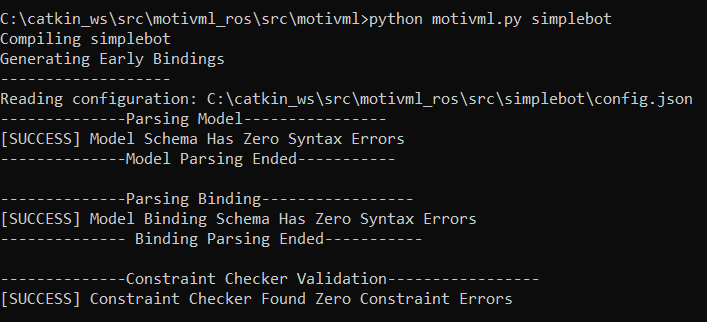
\includegraphics[width=\columnwidth]{images/validate.png}
	\label{validation}
\end{figure}

Upon successful validation without any errors, a \textbf{bindings.motivml} file is generated in the project folder. This file contains features that are have been bound at compile time. At runtime, the \textbf{bindings.motivml} file is dynamically updated depending on which features are successfully bound or unbound.

\subsection{Plug in Source Code Implementations of Model Features}
In the event that there are no syntax and symantic errors detected by the MoTiVML engine, source code implementations of features can be implemented and executed. Source code implementation in both C++ and Python can be plugged in. A source code implementation can be plugged in by following the following steps:

\begin{itemize}
	\item Extract, encapsulate and plug in your feature implementations into the featx directory
	
	\item For each plugged in source code implementation, name the entrypoint file containing the main function with the same name as the corresponding feature in your MoTiVML model.json file.
	
	\item In the MoTiVML commandline interface, a number of commands can be executed to perform specific tasks.
\end{itemize}

\subsection{MoTiVML Console Interface}
To add some interactivity to our variability modelling language, we have provided an in-built console interface for interacting with models and features.

To launch the MoTiVML console interface, navigate to the \textbf{/src/motivml} directory and run the following command in Listing \ref{console}:

\begin{longlisting}
	\caption{MoTiVML Console Launch Command}
	\begin{minted}[
		framesep=2mm,
		baselinestretch=1.2,
		bgcolor=LightGray,
		fontsize=\footnotesize
		]{python}
		
		python mmconsole.py <project_directory_name>
		
	\end{minted}
	\label{console}
\end{longlisting}

Prior to the console interface being launched when the above command is run, the model and configuration of the \textbf{project\_directory\_name} specified in the command is compiled and validated. If there are no errors detected, the console interface is then launched successfully. 

\begin{figure}[H]
	\caption{Simplebot Console}
	\centering
	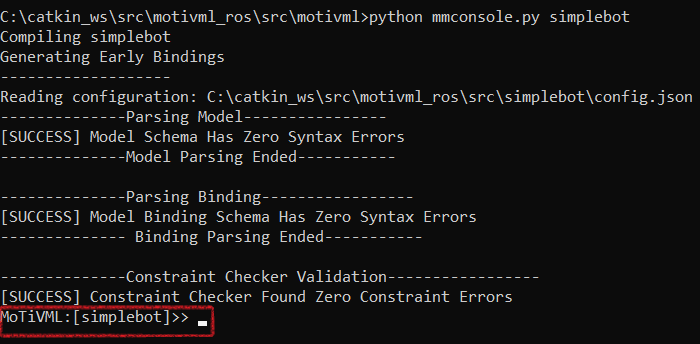
\includegraphics[width=\columnwidth]{images/console.png}
	\label{consolelaunch}
\end{figure}

In Figure \ref{consolelaunch} we can observe the launched MoTiVML console. As highlighted in the figure above, the console prompt always bears the name of the project which was launched with the  console. For this reason, all MoTiVML console commands that are run will be affiliated with the model highlighted in the console prompt.

\subsection{MoTiVML Console Commands}

\begin{itemize}
	\item \textbf{show $<parameter>$}: The show command is used to display graphically a user constructed model. This commands prints the hierarchical structure of a selected model while displaying details such as its mandatory status, group and binding mode. The show command takes a single parameter. This parameter can either be \textbf{all} or  \textbf{config}. \\
	
	The \textbf{show all} command only shows all selected features in the model tree. By default all features are selected when instantiated. Thus, this command shows every single feature in the model tree.
	
	\begin{figure}[H]
		\caption{show all Command}
		\centering
		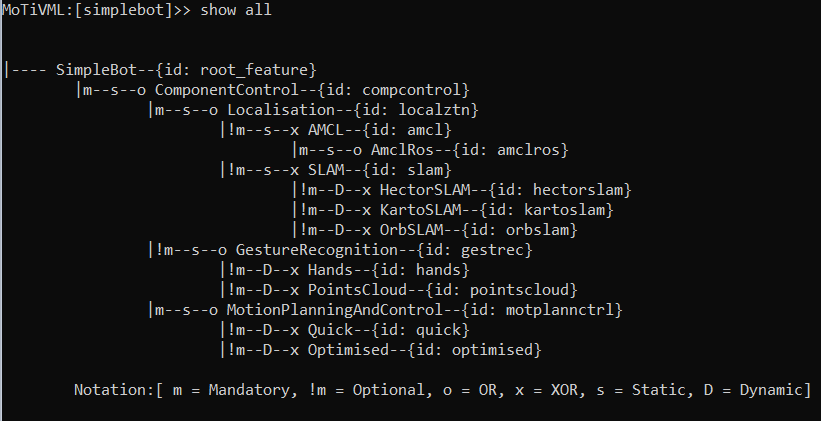
\includegraphics[width=\columnwidth]{images/showall.png}
		\label{showall}
	\end{figure}

	The \textbf{show config} command only shows currently selected features. That is, unselected features i exclude from the output tree.

	\begin{figure}[H]
		\caption{show config Command}
		\centering
		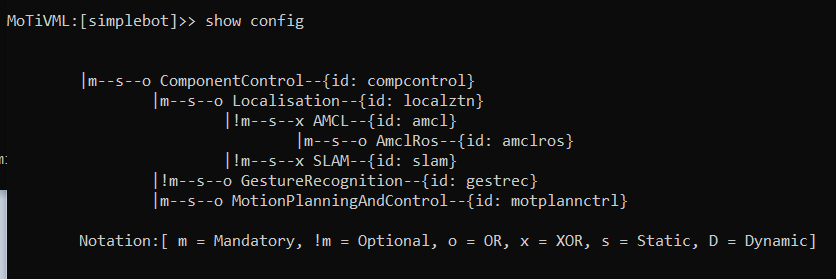
\includegraphics[width=\columnwidth]{images/showconfig.png}
		\label{showconfig}
	\end{figure}

	\item \textbf{run $<feature\_name>$}: The run command executes the source code implementation plugged into a model and linked to a feature in that model. This means that before the run command can be executed successfully, there must be an existing implementation in either C++ or python. The command only takes one parameter which is the name of the feature you wish run.
	
	C++ feature implementation require a compile step to be able to run them. That in the \textbf{src/motivml/featx/mbin} directory of our implementation, we save all C++ feature executables after compilation.
	
	\item \textbf{exit}: The exit command shuts down the console interface and returns back to the original ROS console. The exit command also asks for a yes or no confirmation before proceeding. Figure \ref{exit} shows an exit command execution and output.
	\begin{figure}[H]
		\caption{Exit Command}
		\centering
		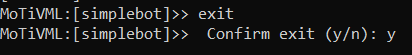
\includegraphics[width=\columnwidth]{images/exit.png}
		\label{exit}
	\end{figure}
\end{itemize}

\end{document}

